%!TEX TS-program = xelatex

\documentclass[a4paper,12pt]{article}

%%% Работа с русским языком
\usepackage[english,russian]{babel}   %% загружает пакет многоязыковой вёрстки
\usepackage{fontspec}      %% подготавливает загрузку шрифтов Open Type, True Type и др.
\defaultfontfeatures{Ligatures={TeX},Renderer=Basic}  %% свойства шрифтов по умолчанию
\setmainfont[Ligatures={TeX,Historic}]{Calibri} %% задаёт основной шрифт документа
\setsansfont{Comic Sans MS}                    %% задаёт шрифт без засечек
\setmonofont{Courier New}
\usepackage{indentfirst}
\frenchspacing

\renewcommand{\epsilon}{\ensuremath{\varepsilon}}
\renewcommand{\phi}{\ensuremath{\varphi}}
\renewcommand{\kappa}{\ensuremath{\varkappa}}
\renewcommand{\le}{\ensuremath{\leqslant}}
\renewcommand{\leq}{\ensuremath{\leqslant}}
\renewcommand{\ge}{\ensuremath{\geqslant}}
\renewcommand{\geq}{\ensuremath{\geqslant}}
\renewcommand{\emptyset}{\varnothing}

%%% Дополнительная работа с математикой
\usepackage{amsmath,amsfonts,amssymb,amsthm,mathtools} % AMS
\usepackage{icomma} % "Умная" запятая: $0,2$ --- число, $0, 2$ --- перечисление

%% Номера формул
%\mathtoolsset{showonlyrefs=true} % Показывать номера только у тех формул, на которые есть \eqref{} в тексте.
%\usepackage{leqno} % Нумерация формул слева	

%% Перенос знаков в формулах (по Львовскому)
\newcommand*{\hm}[1]{#1\nobreak\discretionary{}
	{\hbox{$\mathsurround=0pt #1$}}{}}

%%% Работа с картинками
\usepackage{graphicx}  % Для вставки рисунков
\graphicspath{{images/}}  % папки с картинками
\setlength\fboxsep{3pt} % Отступ рамки \fbox{} от рисунка
\setlength\fboxrule{1pt} % Толщина линий рамки \fbox{}
\usepackage{wrapfig} % Обтекание рисунков текстом

%%% Работа с таблицами
\usepackage{array,tabularx,tabulary,booktabs} % Дополнительная работа с таблицами
\usepackage{longtable}  % Длинные таблицы
\usepackage{multirow} % Слияние строк в таблице
\usepackage{float}% http://ctan.org/pkg/float

%%% Программирование
\usepackage{etoolbox} % логические операторы


%%% Страница
\usepackage{extsizes} % Возможность сделать 14-й шрифт
\usepackage{geometry} % Простой способ задавать поля
\geometry{top=20mm}
\geometry{bottom=20mm}
\geometry{left=30mm}
\geometry{right=15mm}
%
%\usepackage{fancyhdr} % Колонтитулы
% 	\pagestyle{fancy}
%\renewcommand{\headrulewidth}{0pt}  % Толщина линейки, отчеркивающей верхний колонтитул
% 	\lfoot{Нижний левый}
% 	\rfoot{Нижний правый}
% 	\rhead{Верхний правый}
% 	\chead{Верхний в центре}
% 	\lhead{Верхний левый}
%	\cfoot{Нижний в центре} % По умолчанию здесь номер страницы

\usepackage{setspace} % Интерлиньяж
\onehalfspacing % Интерлиньяж 1.5
%\doublespacing % Интерлиньяж 2
%\singlespacing % Интерлиньяж 1

\usepackage{lastpage} % Узнать, сколько всего страниц в документе.

\usepackage{soul} % Модификаторы начертания

\usepackage{hyperref}
\usepackage[usenames,dvipsnames,svgnames,table,rgb]{xcolor}
\hypersetup{				% Гиперссылки
	unicode=true,           % русские буквы в раздела PDF
	pdftitle={Отчет по самостоятельной работе},   % Заголовок
	pdfauthor={Самоделкина М.В., Ремизова А.П.},      % Автор
	pdfsubject={Отчет по самостоятельной работе},      % Тема
	pdfcreator={Самоделкина М.В., Ремизова А.П.}, % Создатель
	pdfproducer={Самоделкина М.В., Ремизова А.П.}, % Производитель
	pdfkeywords={keyword1} {key2} {key3}, % Ключевые слова
	colorlinks=true,       	% false: ссылки в рамках; true: цветные ссылки
	linkcolor=blue,          % внутренние ссылки
	citecolor=black,        % на библиографию
	filecolor=magenta,      % на файлы
	urlcolor=blue           % на URL
}
\makeatletter 
\def\@biblabel#1{#1. } 
\makeatother
\usepackage{cite} % Работа с библиографией
%\usepackage[superscript]{cite} % Ссылки в верхних индексах
%\usepackage[nocompress]{cite} % 
\usepackage{csquotes} % Еще инструменты для ссылок

\usepackage{multicol} % Несколько колонок

\usepackage{tikz} % Работа с графикой
\usepackage{pgfplots}
\usepackage{pgfplotstable}

% ГОСТ заголовки
\usepackage[font=small]{caption}
%\captionsetup[table]{justification=centering, labelsep = newline} % Таблицы по правобу краю
%\captionsetup[figure]{justification=centering} % Картинки по центру
\usepackage{ dsfont }

\newcommand{\tablecaption}[1]{\addtocounter{table}{1}\small \begin{flushright}\tablename \ \thetable\end{flushright}%	
\begin{center}#1\end{center}}

\newcommand{\imref}[1]{рис.~\ref{#1}}

\usepackage{multirow}
\usepackage{spreadtab}
\newcolumntype{K}[1]{@{}>{\centering\arraybackslash}p{#1cm}@{}}


\usepackage{xparse}
\usepackage{fancyvrb}

\RecustomVerbatimCommand{\VerbatimInput}{VerbatimInput}
{
	fontsize=\footnotesize    
}

\newcolumntype{?}[1]{!{\vrule width #1}}

\usepackage{tocloft}
\renewcommand{\cftsecleader}{\cftdotfill{\cftdotsep}}

\usepackage{pdfpages}

\usepackage{longtable}

\usepackage{adjustbox}
\begin{document}
\begin{titlepage}
	\begin{center}
		ПРАВИТЕЛЬСТВО РОССИЙСКОЙ ФЕДЕРАЦИИ \\
 		ФЕДЕРАЛЬНОЕ  ГОСУДАРСТВЕННОЕ АВТОНОМНОЕ \\
		ОБРАЗОВАТЕЛЬНОЕ УЧРЕЖДЕНИЕ ВЫСШЕГО ОБРАЗОВАНИЯ\\
		«НАЦИОНАЛЬНЫЙ ИССЛЕДОВАТЕЛЬСКИЙ УНИВЕРСИТЕТ\\
		«ВЫСШАЯ ШКОЛА ЭКОНОМИКИ»
	\end{center}
	
	\begin{center}
		\textbf{Московский институт электроники и математики}
		
		\textbf{Им. А.Н.Тихонова НИУ ВШЭ}
		
		\vspace{2ex}
		
		\textbf{Направление 01.03.04. Прикладная математика \\
			Бакалаврская программа <<Прикладная математика>>}
	\end{center}
	\vspace{1ex}	
	
	\vspace{1ex}
	\begin{center}
		\textbf{Отчет по самостоятельной работе \\
			по дисциплине <<Методы анализа стохастических взаимосвязей>>\\
			часть 2
	}
	\end{center}	

	\vspace{2ex}
	\vfill
	
	\vspace{2ex}
	
	\begin{flushright}
		\textbf{Бригада №7:}
		
		\vspace{2ex}
		
		Ремизова Анна Петровна, 4 курс, БПМ174
		
		Самоделкина Мария Владимировна, 4 курс, БПМ174

	\end{flushright}

	\vspace{5ex}
	\begin{center}
		Москва \the\year \, г.
	\end{center}
	
\end{titlepage}
\addtocounter{page}{1}
\tableofcontents
\pagebreak

\section{Описание данных}
% Период времени и тип данных
Частота измерений каждые 4 секунды. Величину стандартного интервала наблюдений принимаем равным одной минуте (содержит 15 измерений). 15 наблюдений откладываем для проверки прогностической способности моделей.

% Гипотезы

\subsection{Зависимая переменная Пульс}
% Определение
\begin{figure}[H]
	\centering
	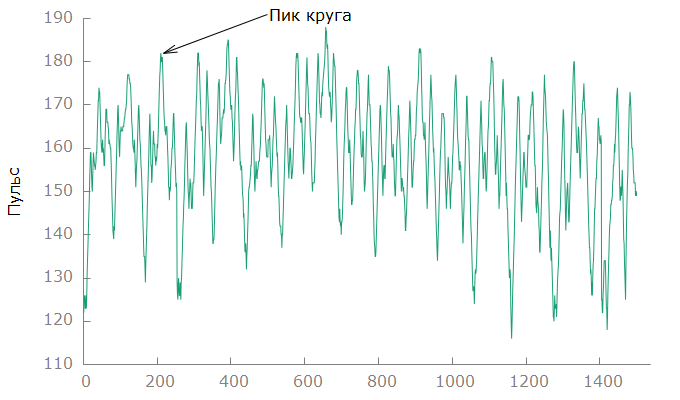
\includegraphics[width=0.7\linewidth]{../[graphics]/hr_graph}
	\caption{График зависимой переменной Пульс}
	\label{fig:hr_graph}
\end{figure}

% Анализ автокорреляции
\textbf{\textit{Анализ автокорреляции}}

\begin{figure}[H]
	\centering
	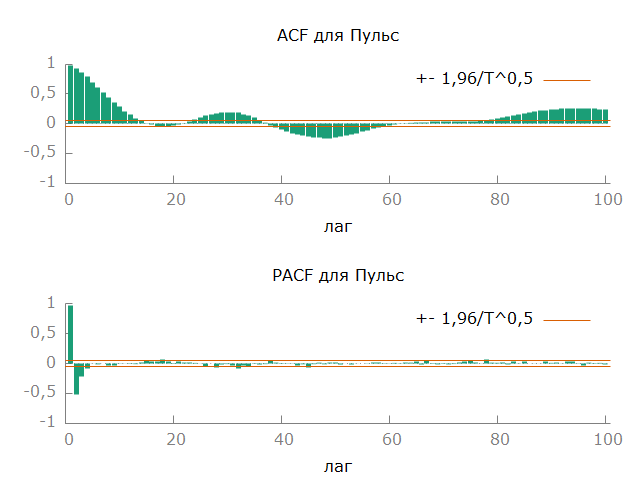
\includegraphics[width=0.7\linewidth]{../[graphics]/hr_acf_100}
	\caption{Графики ACF и PACF зависимой переменной Пульс}
	\label{fig:hr_acf_100}
\end{figure}

График автокорреляции (рис. \ref{fig:hr_acf_100}) убывает медленно, предполагается наличие тренда. На графике видны колебания с периодом в 2 минуты (лаг 30), 3 минуты (лаг 45) и 6 минут (лаг 88). При анализе графика значений зависимой переменной (рис. \ref{fig:hr_graph}) также хорошо видны колебания в 6 минут. По виду графиков можно говорить о наличии циклического тренда с периодом, равным среднему времени прохождения спортсменом круга (около 6 минут).

% Анализ спектрограммы
\textbf{\textit{Анализ спектрограммы}}

\begin{figure}[H]
	\centering
	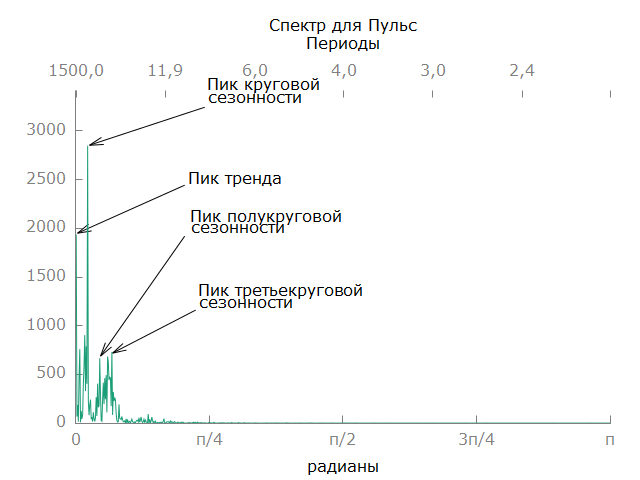
\includegraphics[width=0.7\linewidth]{../[graphics]/hr_spectr}
	\caption{График периодограммы зависимой переменной Пульс}
	\label{fig:hr_spectr}
\end{figure}

При анализе графика (рис. \ref{fig:hr_spectr}) видны пики вблизи нулевой частоты, они свидетельствуют о потенциальном наличии долгосрочного тренда. На графике также видны несколько пиков в циклической области спектра. 
В циклической части спектра на частоте $f = 0,07193 \approx \frac{2 \pi}{87}$ значение спектральной частоты равно $Sd = 2814,4$, указанная частота соответствует периоду 6 минут (среднее время прохождения одного круга).
На частоте $f = 0,20309 \approx \frac{2 \pi}{31}$ значение спектральной частоты равно $Sd = 1167,8$, указанная частота соответствует периоду в 2 минуты (треть круга).
Пиков в сезонной части спектра нет. 
Гармоническая составляющая в указанном ряду является хорошо выраженной.

% Анализ стационарности с использованием критерия Dickey-Fuller

%Выводы
\textbf{\textit{Выводы}}

Наличие долгосрочного тренда зависимой переменной Пульса объясняется тем, что с течением времени тренировки спортсмен устает, вследствие чего пульс постепенно увеличивается. Наличие циклического тренда в 6 минут объясняется тем, что рельеф местности каждый круг повторяется. Наличие циклической частоты с периодом, равным в 2 минуты (треть круга) связано с периодичной сменой техники передвижения. %TODO

\subsection{Независимые переменные}
\subsubsection{Высота}
% Определение
\begin{figure}[H]
	\centering
	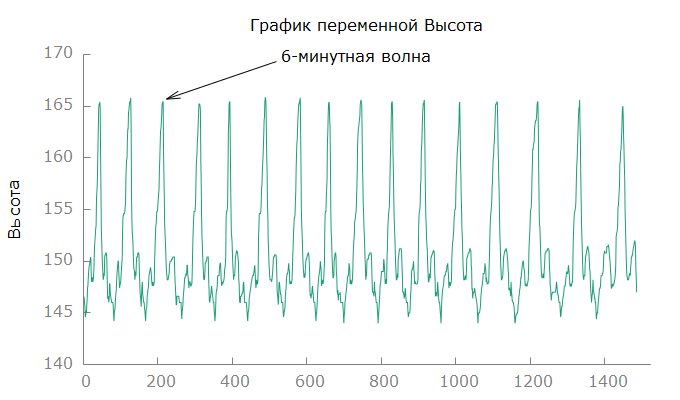
\includegraphics[width=0.7\linewidth]{../[graphics]/ele_graph}
	\caption{График зависимой Высота}
	\label{fig:ele_graph}
\end{figure}

% Анализ автокорреляции
\textbf{\textit{Анализ автокорреляции}}

\begin{figure}[H]
	\centering
	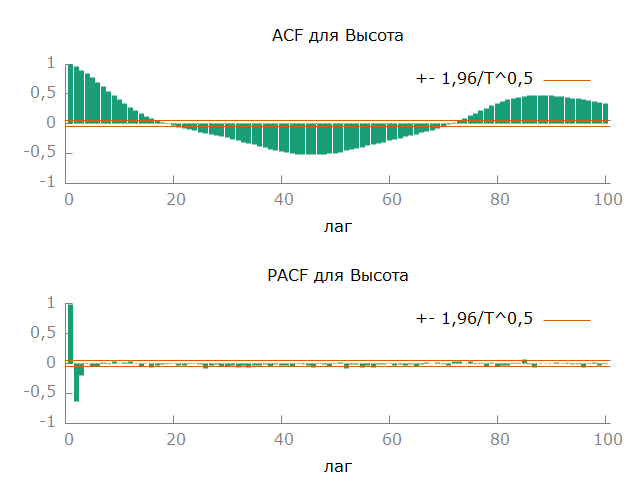
\includegraphics[width=0.7\linewidth]{../[graphics]/ele_acf_100}
	\caption{Графики ACF и PACF переменной Высота}
	\label{fig:ele_acf_100}
\end{figure}

График автокорреляции (рис. \ref{fig:ele_acf_100}) убывает медленно, предполагается наличие тренда. На графике видны колебания с периодом полкруга (3 минуты) и круг (6 минут). При анализе графика значений переменной (рис. \ref{fig:ele_graph}) также хорошо видны колебания с периодом в 6 минут. По виду графиков можно говорить о наличии циклического тренда с периодом, равным среднему времени прохождения спортсменом круга.

% Анализ спектрограммы
\textbf{\textit{Анализ спектрограммы}}

\begin{figure}[H]
	\centering
	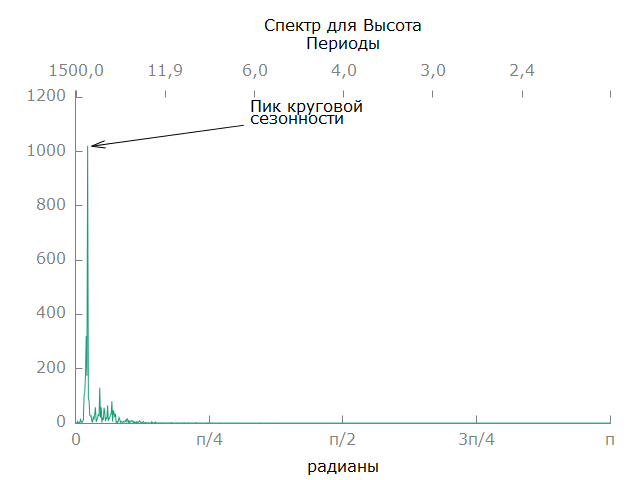
\includegraphics[width=0.7\linewidth]{../[graphics]/ele_spectr}
	\caption{График периодограммы переменной Высота}
	\label{fig:ele_spectr}
\end{figure}

При анализе графика (рис. \ref{fig:hr_spectr}) видно, что пики вблизи нулевой частоты отсутствуют, долгосрочного тренда нет. На графике отсутствуют пики в сезонной области спектра. 
В циклической части спектра на частоте $f = 0,07193 \approx \frac{2 \pi}{87}$ значение спектральной частоты равно $Sd = 938,12$, указанная частота соответствует периоду в 6 минут. 
В циклической части спектра на частоте $f = 0,14386 \approx \frac{2 \pi}{44}$ значение спектральной частоты равно $Sd = 129,12$, указанная частота соответствует периоду в 3 минуты.
В циклической части спектра на частоте $f = 0,22425 \approx \frac{2 \pi}{28}$ значение спектральной частоты равно $Sd = 97,627$, указанная частота соответствует периоду в 2 минуты.
У данного ряда есть ярковыраженная циклическая составляющая.
Также имеются другие неярковыраженные пики в циклической части спектра.

% Анализ стационарности с использованием критерия Dickey-Fuller

%Выводы
\textbf{\textit{Выводы}}

Долгосрочного тренда в рассматриваемом ряде быть не должно: спортсмен каждый круг проезжал по одной и той же территории, высота не изменялась. 
Однако заметен циклический тренд с периодом в 6 минут. Наличие циклического тренда объясняется тем, что рельеф местности каждый круг повторяется. Однако в изменениях высоты могут присутствовать незначительные колебания из-за того, что спортсмен каждый раз мог выбирать незначительно отличающуюся траекторию.

\subsubsection{Каденс}
% Определение
\begin{figure}[H]
	\centering
	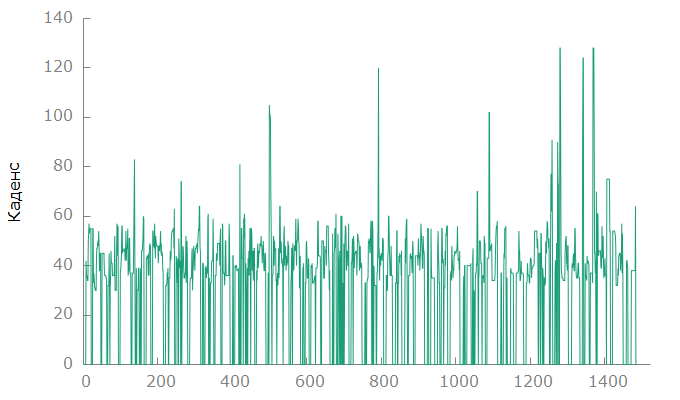
\includegraphics[width=0.7\linewidth]{../[graphics]/cad_graph}
	\caption{График зависимой Каденс}
	\label{fig:cad_graph}
\end{figure}

% Анализ автокорреляции
\textbf{\textit{Анализ автокорреляции}}

\begin{figure}[H]
	\centering
	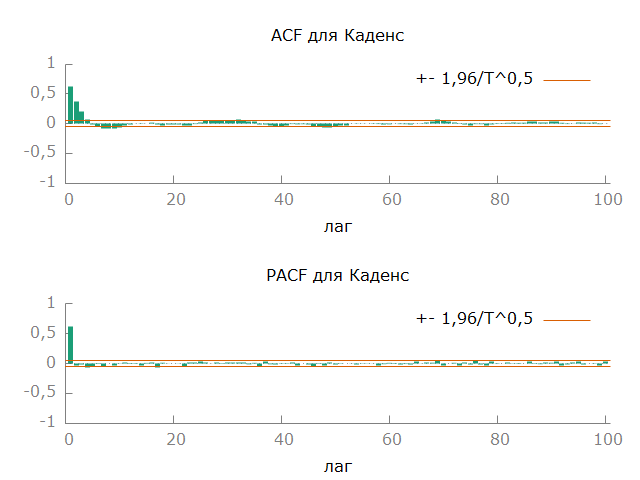
\includegraphics[width=0.7\linewidth]{../[graphics]/cad_acf_100}
	\caption{Графики ACF и PACF переменной Каденс}
	\label{fig:cad_acf_100}
\end{figure}

График автокорреляции (рис. \ref{fig:cad_acf_100}) убывает быстро, предполагается отсутствие тренда. Влияние сезонности предположительно отсутствует. Указанные замечания также соотносятся с графиком значений переменной (рис. \ref{fig:cad_graph}).

% Анализ спектрограммы
\textbf{\textit{Анализ спектрограммы}}

\begin{figure}[H]
	\centering
	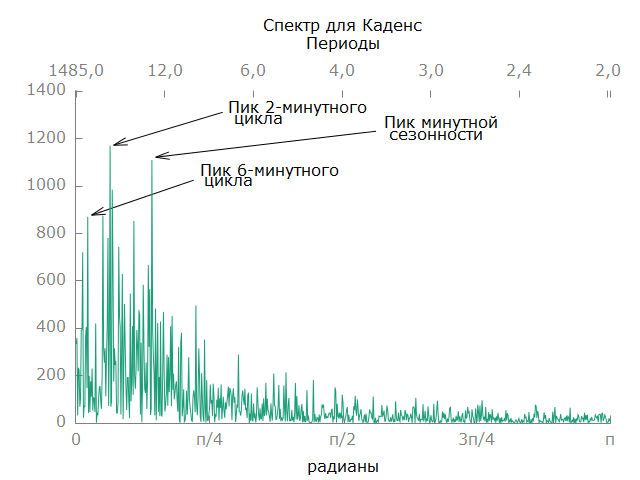
\includegraphics[width=0.7\linewidth]{../[graphics]/cad_spectr}
	\caption{График периодограммы переменной Каденс}
	\label{fig:cad_spectr}
\end{figure}

При анализе графика (рис. \ref{fig:cad_spectr}) видно, что пики вблизи нулевой частоты отсутствуют, долгосрочного тренда нет. На графике присутствуют пики в циклической области спектра. 
В циклической части спектра на частоте $f = 0,07193 \approx \frac{2 \pi}{87}$ значение спектральной частоты равно $Sd = 870,59$, указанная частота соответствует периоду в 6 минут.
В циклической части спектра на частоте $f = 0,20309 \approx \frac{2 \pi}{31}$ значение спектральной частоты равно $Sd = 1170,6$, указанная частота соответствует периоду в 2 минуты.
В сезонной части спектра на частоте $f = 0,44850 \approx \frac{2 \pi}{14}$ значение спектральной частоты равно $Sd = 1110,2$, указанная частота соответствует периоду в 1 минуту.
Также имеются другие пики в циклической и сезонной частях спектра.

% Анализ стационарности с использованием критерия Dickey-Fuller

%Выводы
\textbf{\textit{Выводы}}

Отсутствие тренда связано с тем, что используемая в конкретный момент техника передвижения спортсмена практически не зависит от техники, используемой в предыдущие моменты времени.
Наличие сезонных частот с периодами в 1 и 2 минуты связано с периодичностью применяемой техники передвижения. %TODO

\subsubsection{Сезонные переменные}
Анализ зависимой переменной не выявил наличие гармонических составляющих с периодами, меньшими минуты.

\section{Выделение трендов}
Начнем с выделения циклических трендов, поскольку они наиболее ярко просматриваются на графиках переменных.

\subsection{Удаление циклического тренда}
Для удаления циклических трендов будем использовать гармонические функции. Из анализа спектрограммы следует, что в рядах присутствуют периодические составляющие с периодами 6 минут, 3 минуты, 2 минуты и 1 минута. Также рассматриваются дополнительные частоты, в которых спектральная частота принимает большие значения. Всего было выявлено 14 частот, в которых замечены высокие значения спектральной частоты (далее нумерация введенных переменных-гармоник соответствует указанному порядку): $$\frac{2 \pi}{297}, \frac{2 \pi}{248}, \frac{2 \pi}{124}, \frac{2 \pi}{114}, \frac{2 \pi}{106}, \frac{2 \pi}{99}, \frac{2 \pi}{93}, \frac{2 \pi}{87}, \frac{2 \pi}{44}, \frac{2 \pi}{36}, \frac{2 \pi}{33}, \frac{2 \pi}{31}, \frac{2 \pi}{28}, \frac{2 \pi}{14}.$$

\subsubsection{Зависимая переменная Пульс}
Построим линейную регрессию переменной Пульс на гармониках для указанных выше частот. Результаты расчетов приведены в таблице ниже. Нами использовались робастные стандартные ошибки HAC. %TODO.
Все частоты за исключением $\frac{2 \pi}{14}$ получились значимыми.

\begin{table}[H]
\begin{center}
	
	Удаление циклического тренда зависимой переменной: МНК, использованы наблюдения 1--1485\\
	Зависимая переменная: ns2hr\\
	Стандартные ошибки HAC, ширина окна 8 (Ядро Бартлетта (Bartlett))
	
	\vspace{1em}
	
	\begin{tabular}{lr@{,}lr@{,}lr@{,}lr@{,}l}
		&
		\multicolumn{2}{c}{Коэффициент} &
		\multicolumn{2}{c}{Ст.\ ошибка} &
		\multicolumn{2}{c}{$t$-статистика} &
		\multicolumn{2}{c}{P-значение} \\[1ex]
		const &		157&743 &		0&656379 &		240&3 &		0&0000 \\
		c1 &		0&00308109 &		0&775609 &		0&003972 &		0&9968 \\
		s1 &		2&96469 &		1&06039 &		2&796 &		0&0052 \\
		c2 &		$-$3&45727 &		0&887961 &		$-$3&893 &		0&0001 \\
		s2 &		$-$0&451657 &		0&973332 &		$-$0&4640 &		0&6427 \\
		c3 &		2&15391 &		0&921646 &		2&337 &		0&0196 \\
		s3 &		$-$2&14060 &		0&900929 &		$-$2&376 &		0&0176 \\
		c4 &		0&0245971 &		0&900507 &		0&02731 &		0&9782 \\
		s4 &		$-$3&77913 &		0&940082 &		$-$4&020 &		0&0001 \\
		c5 &		$-$1&86244 &		0&969532 &		$-$1&921 &		0&0549 \\
		s5 &		$-$1&60608 &		0&885599 &		$-$1&814 &		0&0700 \\
		c6 &		0&445651 &		0&903548 &		0&4932 &		0&6219 \\
		s6 &		3&29686 &		0&951217 &		3&466 &		0&0005 \\
		c7 &		1&21006 &		0&841936 &		1&437 &		0&1509 \\
		s7 &		3&48608 &		0&985024 &		3&539 &		0&0004 \\
		c8 &		$-$6&15996 &		0&870829 &		$-$7&074 &		0&0000 \\
		s8 &		$-$3&03899 &		0&929493 &		$-$3&270 &		0&0011 \\
		c9 &		$-$1&63113 &		0&899804 &		$-$1&813 &		0&0701 \\
		s9 &		$-$2&23476 &		0&881073 &		$-$2&536 &		0&0113 \\
		c10 &		1&71114 &		0&806446 &		2&122 &		0&0340 \\
		s10 &		$-$3&52976 &		0&901322 &		$-$3&916 &		0&0001 \\
		c11 &		$-$3&48449 &		0&887674 &		$-$3&925 &		0&0001 \\
		s11 &		$-$2&09333 &		0&830548 &		$-$2&520 &		0&0118 \\
		c12 &		1&54375 &		0&853418 &		1&809 &		0&0707 \\
		s12 &		$-$4&16356 &		0&822035 &		$-$5&065 &		0&0000 \\
		c13 &		$-$2&13518 &		0&839731 &		$-$2&543 &		0&0111 \\
		s13 &		$-$2&01712 &		0&806885 &		$-$2&500 &		0&0125 \\
		c14 &		0&900906 &		0&576660 &		1&562 &		0&1184 \\
		s14 &		0&213285 &		0&571939 &		0&3729 &		0&7093 \\
	\end{tabular}
	
	\vspace{1ex}
	\begin{tabular}{lrlr}
		Среднее зав. перемен &  157,6983 & Ст. откл. зав. перемен &  13,68422 \\
		Сумма кв. остатков &  137168,6 & Ст. ошибка модели &  9,706143 \\
		$R^2$ &  0,506394 & Исправленный $R^2$ &  0,496901 \\
		$F(28, 1456)$ &  17,73434 & Р-значение($F$) &  9,59\textrm{e--74} \\
		Лог. правдоподобие & $-$5467,527 & Крит. Акаике &  10993,05 \\
		Крит. Шварца &  11146,85 & Hannan--Quinn &  11050,38 \\
		$\hat{\rho}$ &  0,963471 & Durbin--Watson &  0,072530 \\
	\end{tabular}
\end{center}
\caption{Удаление циклического тренда зависимой переменной Пульс с корректировкой на автокорреляцию.}
\label{tab:table1}
\end{table}

Графики расчетных значений модели и остаточной разности представлены соответственно на рис.\ref{fig:hr_trend0} и рис.\ref{fig:hr_error0}.

\begin{figure}[H]
	\centering
\begin{minipage}{.5\textwidth}
	\centering
	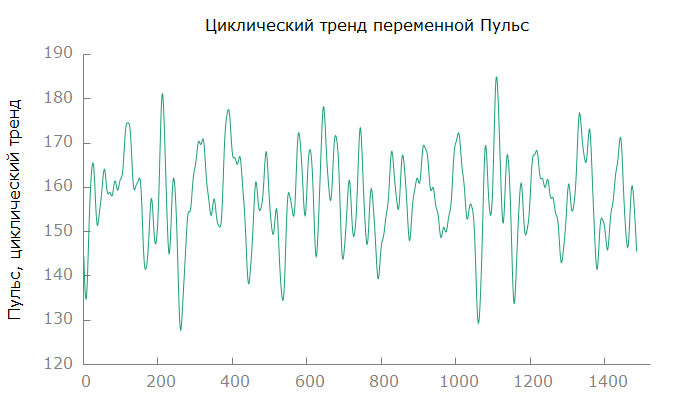
\includegraphics[width=\linewidth]{../[graphics]/hr_trend0.png}
	\caption{Циклический тренд переменной Пульс}
	\label{fig:hr_trend0}
\end{minipage}%
\begin{minipage}{.5\textwidth}
	\centering
	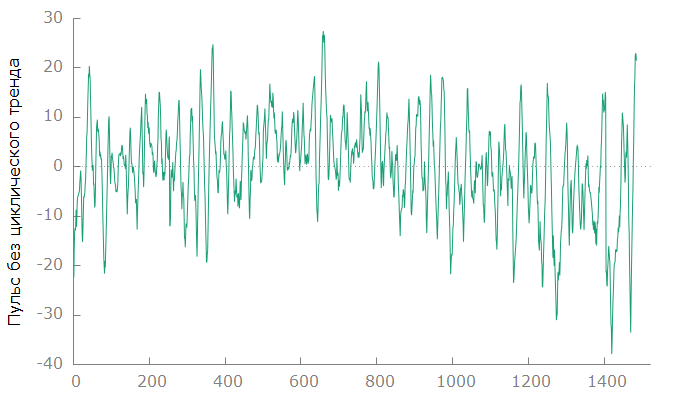
\includegraphics[width=\linewidth]{../[graphics]/hr_error0.png}
	\caption{Пульс без циклического тренда}
	\label{fig:hr_error0}
\end{minipage}
\end{figure}

По графику спектра переменной Пульс без циклического тренда (рис.\ref{fig:hr_error0_spectr}) видно, что мы действительно избавились от циклической составляющей.

\begin{figure}[H]
	\centering
	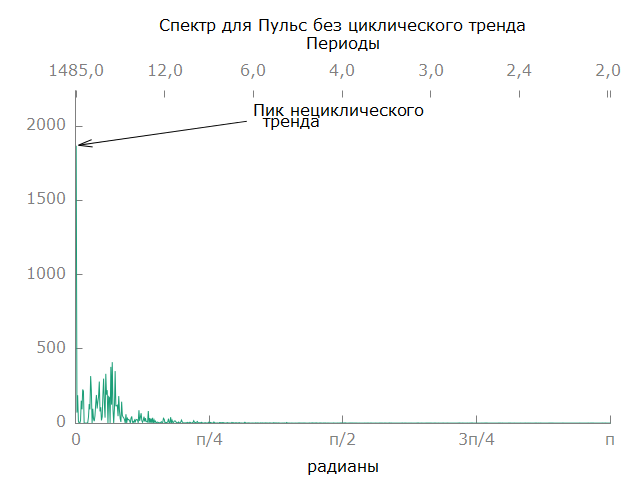
\includegraphics[width=0.7\linewidth]{../[graphics]/hr_error0_spectr.png}
	\caption{График спектра переменной Пульс без циклического тренда}
	\label{fig:hr_error0_spectr}
\end{figure}

Для дальнейшего анализа будем использовать остаточную разность hr\_error0, полученную из переменной Пульс после удаления циклического тренда.

\subsubsection{Независимые переменные}
Аналогично предыдущему пункту построим линейные регрессии для независимых переменных Высота и Каденс на указанных ранее гармониках. 
Для переменной Высота все частоты кроме $\frac{2 \pi}{248}, \frac{2 \pi}{14}$ получились значимыми. Для переменной Каденс значимыми оказались частоты $\frac{2 \pi}{106}, \frac{2 \pi}{99}, \frac{2 \pi}{87}, \frac{2 \pi}{44}, \frac{2 \pi}{33}, \frac{2 \pi}{31}, \frac{2 \pi}{14}$.

По графику спектра переменной Высота без циклического тренда (рис.\ref{fig:ele_error0_spectr}) видно, что пиков стало меньше, но окончательно избавиться от циклической составляющей не удалось.

\begin{figure}[H]
	\centering
	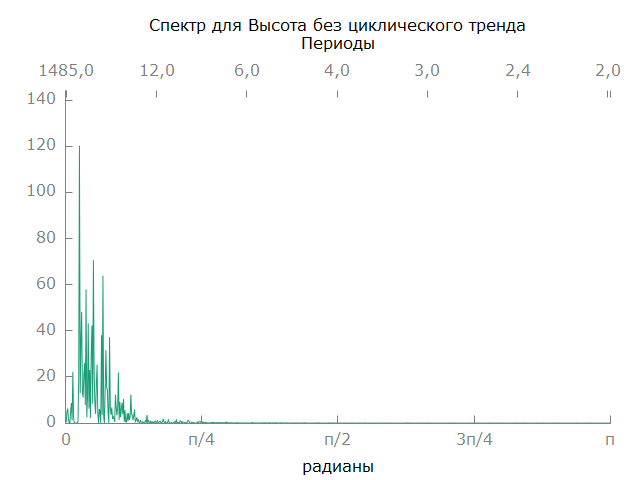
\includegraphics[width=0.7\linewidth]{../[graphics]/ele_error0_spectr.png}
	\caption{График спектра переменной Высота без циклического тренда}
	\label{fig:ele_error0_spectr}
\end{figure}

По графику спектра переменной Каденс без циклического тренда (рис.\ref{fig:cad_error0_spectr}) видно, что пиков стало меньше, но окончательно избавиться от циклической составляющей не удалось.

\begin{figure}[H]
	\centering
	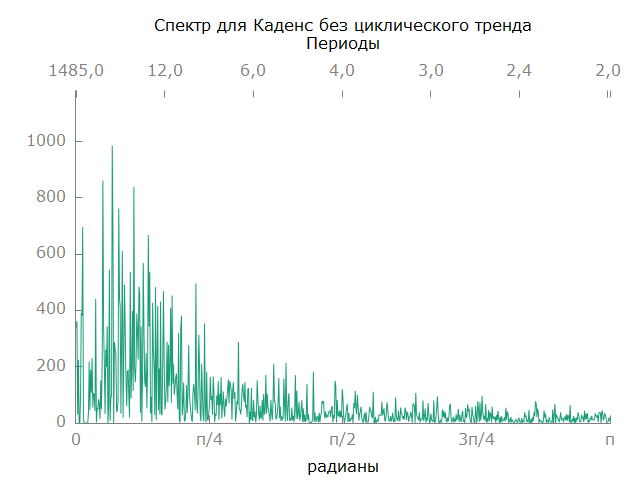
\includegraphics[width=0.7\linewidth]{../[graphics]/cad_error0_spectr.png}
	\caption{График спектра переменной Каденс без циклического тренда}
	\label{fig:cad_error0_spectr}
\end{figure}

Для дальнейшего анализа будем использовать остаточные разности ele\_error0 и cad\_error0, полученные соответственно из переменных Высота и Каденс после удаления циклического тренда.


\end{document} % конец документа